\section{Magnetoquasistatische Analyse (MQS, Magnetoquasistatic Analysis)}
Die magnetoquasistatische Analyse wird gebraucht um bei Wechselstrom die Ersatzwiderstände eines Gerätes zu berechnen. Weil es sich um langsam ändernde Felder handelt muss der Verschiebungsstrom von Maxwell nicht beachtet werden.  
\subsection{Integralgleichungen}
\begin{tabular}{|p{.30\textwidth} |p{.65\textwidth}|}
	\hline 
	\textbf{Ampèresches Gesetz} \newline
	{\centering\tabbild[width=4cm]{images/ampgesetz.png}\par} & Das Ampèresche Gesetz definiert die Verteilung des magnetischen Feldes durch eine geschlossene Kurve ist der gesamte Strom durch die entsprechende Fläche
	\[ \oint\limits_{(C)}\vec{H}\cdot\vec{dl} = \sum_{k=1}^n I_k =\iint\limits_{(A)}\vec{J}\cdot\vec{dA}\] \newline
	\[ \oint\limits_{(C)}\vec{B}\cdot\vec{dl} = \mu_{0}\iint\limits_{(A)}\vec{J}\cdot\vec{dA} \quad \quad\vec{B}=\mu_{0}\mu_{r}\cdot \vec{H}\]\\
	\hline
	\textbf{Coulombsches Gesetz} \newline
	{\centering\tabbild[width=4cm]{images/quellenfreiheit.png}\par} & Der magnetische Fluss durch eine geschlossene Fläche ist immer Null. Somit sind die magnetische Feldlinien immer geschlossen. Es gibt keine magnetische Monopole. Das magnetische Feld ist Quellenfrei \newline
	\[ \oiint\limits_{(A)}\vec{B}\cdot\vec{dA} = 0\]\\
	\hline
	\textbf{Faradaysches Induktionsgesetz}
	{\centering\tabbild[width=4cm]{images/faradaygesetz.png}\par} & Der zeitabhängige magnetische Fluss induziert elektrische Spannung in der vom Fluss durchflossenen Spule.\newline
	\[u_{i}=-\frac{\partial \Phi_{m}}{\partial t}\] \newline
	\[\Phi_{m}=\oiint\limits_{(S)} \vec{B}\cdot \vec{dS}\quad und \quad u_{i}=\oint \limits_{(C)}\vec{E}\cdot \vec{dl}\]\newline
	\[\oint \limits_{(C)}\vec{E}\cdot \vec{dl}= - \frac{\partial}{\partial t} \oiint\limits_{(S)} \vec{B}\cdot \vec{dS}\]\\
	\hline
\end{tabular}
\clearpage
\pagebreak
\subsection{Differenzialgleichungen der magnetoquasostatischen Analyse}
\begin{tabular}{|p{.45\textwidth} |p{.45\textwidth}|}
	\hline
	\textbf{Differenzialgleichung der Durchflutung}\newline
	\[\rotation \vec{H}=\nabla \times \vec{H}=\vec{J}\]
	\[\rotation \vec{B}=\nabla \times \vec{B}=\mu_{0}\vec{J}\] \vspace{1cm} \[\vec{J} = \vec{J_q} + \vec{J_i}\] 
	{\begin{align*}
		\vec{J} &= \vec{J_q} + \sigma\vec{E_i} \\
		&= \vec{J_q} -\sigma\dfrac{\partial\vec{A}}{\partial t}\\
		&= \vec{J_q} - j\omega\sigma A
	\end{align*}} \vspace{-1cm}&
	\textbf{Vektorpotential}\newline
	Die Stromdichte besteht aus dem statischen Teil und dem induzierten Teil\newline
	$J_i=\sigma \cdot E_i $ \qquad``statisch''\newline
	$\vec{E_i}=-\dfrac{\partial \vec{A}}{\partial t}$ \qquad ``induziert''\newline \newline
	$ \left. \begin{array}{c} \Delta\vec{A}-\mu_{0}\sigma \dfrac{\partial \vec{A}}{\partial t}=-\mu_{0}\vec{J}\\\Delta\vec{A}-j\omega\mu_{0}\sigma\vec{A}=-\mu_{0}\vec{J} \end{array} \right\}$ Im Leiter\newline \newline \newline 
		$ \left. \begin{array}{c} \Delta\vec{A}-\mu_{0}\sigma \dfrac{\partial \vec{A}}{\partial t}=0\\\Delta\vec{A}-j\omega\mu_{0}\sigma\vec{A}=0 \end{array} \qquad \right\}$ Ausserhalb des Leiters\\
		& \\
	\hline
\end{tabular}
\subsection{Randbedingungen}
\begin{itemize}
	\item Magnetische Isolierung $\vec{n} \times \vec{A} =0$
	\item Der Rand zwischen zwei Materialien $\vec{n} \times \vec{A_{1}}=\vec{n} \times \vec{A_{2}}$
	\item Der Rand zwischen zwei Materialien $B_{1}=B_{2} \rightarrow \dfrac{dA_{1}}{d n}=\dfrac{dA_{2}}{d n} $
\end{itemize}
\subsection{Randwertproblem}
\begin{minipage}{9cm}
	\begin{itemize}
		\item Zeitbereich: $\Delta\vec{A}-\mu_{0}\sigma \dfrac{\partial \vec{A}}{\partial
		 t}=-\mu_{0}\vec{J}$
		\item Frequenzbereich: $\Delta\vec{A}-j\omega\mu_{0}\sigma\vec{A}=-\mu_{0}\vec{J}$
		\item $\vec{n} \times \vec{A} =0$
	\end{itemize}	
\end{minipage}
\begin{minipage}{8cm}
	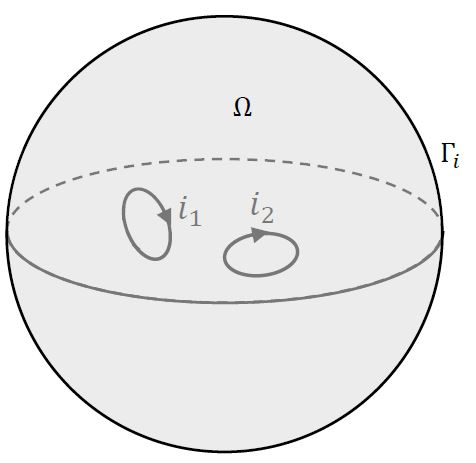
\includegraphics[width=4cm]{images/Randwertproblem.jpg}
\end{minipage}
\subsection{Vorgehen}
	\begin{enumerate}
		\item Partielle Differentialgleichung 2. Ordnung des Vektorpotentials aufstellen (Poisson oder Laplace)
		\item Vereinfachung der partiellen DGL
		\subitem Von welcher Variable hängt das Vektorpotential ab
		\subitem $\dfrac{\partial \vec{A}}{\partial t}= j\omega\vec{A} $
		\item Aufstellen der Randbedingungen
		\subitem Randwerte für Vektorpotential und B-Feld
		\item Welche Form hat die DGL 
		\subitem Homogen $\ddot{f}(x) - f(x)=0$
		\subitem Inhomogen $\ddot{f}(x) - f(x)=C$
		\item DGL mittels Ansatz über Homogene und Partikuläre Lösung $Y=Y_{H}+Y_{P}$
		\subitem Homogene Lösung: Charakteristisches Polynom
		\subitem Partikuläre Lösung: Mittels Störterm, K ist konstant und einsetzen
	\end{enumerate}
\clearpage
\pagebreak
